
\chapter{Implementation}
\label{chap:implementation}
% logo definitions
\newcommand{\logoFleur}{%
  \begingroup\normalfont
  
\includegraphics[height=1.2\fontcharht\font`\B]{img/logo/fleur.png}%
  \endgroup
}
\newcommand{\logoAiida}{%
  \begingroup\normalfont
  
\includegraphics[height=1.0\fontcharht\font`\B]{img/logo/aiida.png}%
  \endgroup
}
\newcommand{\logoAiidalab}{%
  \begingroup\normalfont
  
\includegraphics[height=1.0\fontcharht\font`\B]{img/logo/aiidalab.png}%
  \endgroup
}
\newcommand{\logoBinder}{%
  \begingroup\normalfont
  
\includegraphics[height=1.2\fontcharht\font`\B]{img/logo/binder.png}%
  \endgroup
}
\newcommand{\logoBokeh}{%
  \begingroup\normalfont
  
\includegraphics[height=1.2\fontcharht\font`\B]{img/logo/bokeh.png}%
  \endgroup
}
\newcommand{\logoDash}{%
  \begingroup\normalfont
  
\includegraphics[height=1.2\fontcharht\font`\B]{img/logo/dash.png}%
  \endgroup
}
\newcommand{\logoDocker}{%
  \begingroup\normalfont
  
\includegraphics[height=1.2\fontcharht\font`\B]{img/logo/docker.png}%
  \endgroup
}
\newcommand{\logoHoloviews}{%
  \begingroup\normalfont
  
\includegraphics[height=1.2\fontcharht\font`\B]{img/logo/holoviews.png}%
  \endgroup
}
\newcommand{\logoHvplot}{%
  \begingroup\normalfont
  
\includegraphics[height=1.2\fontcharht\font`\B]{img/logo/hvplot.png}%
  \endgroup
}
\newcommand{\logoJavascript}{%
  \begingroup\normalfont
  
\includegraphics[height=1.2\fontcharht\font`\B]{img/logo/javascript.png}%
  \endgroup
}
\newcommand{\logoJupyter}{%
  \begingroup\normalfont
  
\includegraphics[height=1.2\fontcharht\font`\B]{img/logo/jupyter.png}%
  \endgroup
}
\newcommand{\logoMatplotlib}{%
  \begingroup\normalfont
  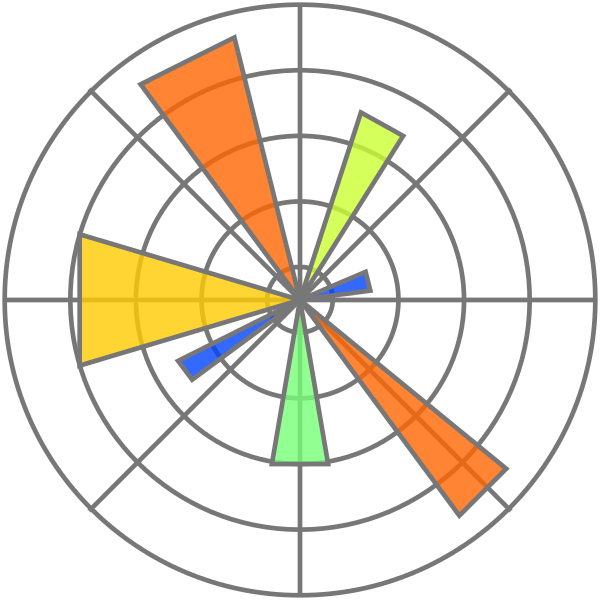
\includegraphics[height=1.2\fontcharht\font`\B]{img/logo/matplotlib.png}%
  \endgroup
}
% \newcommand{\logoMpld3}{%
%   \begingroup\normalfont
%   
\includegraphics[height=1.2\fontcharht\font`\B]{img/logo/mpld3.png}%
%   \endgroup
% }
\newcommand{\logoPanel}{%
  \begingroup\normalfont
  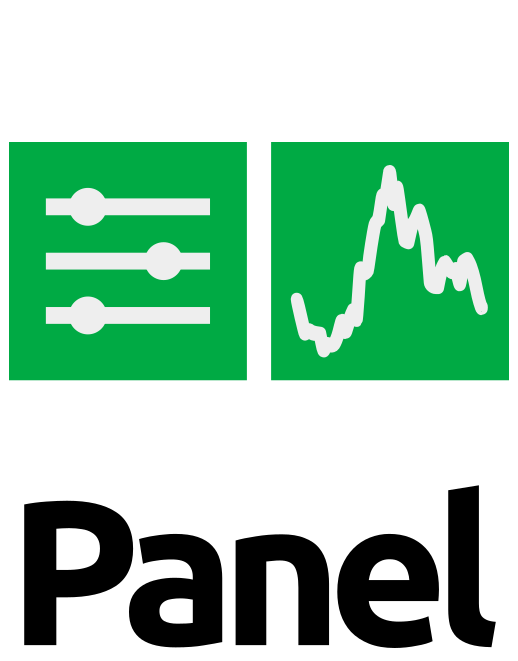
\includegraphics[height=1.2\fontcharht\font`\B]{img/logo/panel.png}%
  \endgroup
}
\newcommand{\logoParam}{%
  \begingroup\normalfont
  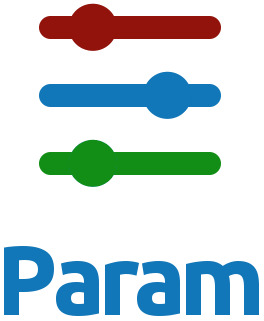
\includegraphics[height=1.2\fontcharht\font`\B]{img/logo/param.png}%
  \endgroup
}
\newcommand{\logoPlotly}{%
  \begingroup\normalfont
  
\includegraphics[height=1.2\fontcharht\font`\B]{img/logo/plotly.png}%
  \endgroup
}
\newcommand{\logoPython}{%
  \begingroup\normalfont
  
\includegraphics[height=1.2\fontcharht\font`\B]{img/logo/python.png}%
  \endgroup
}
\newcommand{\logoPyviz}{%
  \begingroup\normalfont
  
\includegraphics[height=1.2\fontcharht\font`\B]{img/logo/pyviz.png}%
  \endgroup
}
\newcommand{\logoSeaborn}{%
  \begingroup\normalfont
  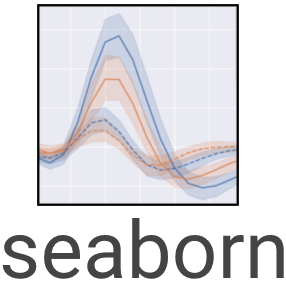
\includegraphics[height=1.2\fontcharht\font`\B]{img/logo/seaborn.png}%
  \endgroup
}

%%% Local Variables:
%%% mode: latex
%%% TeX-master: t
%%% End:


As per the requirements expounded upon in the introduction, the deliverable of
the project should be a finished software product. The software is written in
Python so as to integrate easily with the research group's ongoing software
projects around the Fleur code \cite{fleur}. These are chiefly the group's
materials science tool collection \texttt{masci-tools} \cite{masci-tools} ,
where also this project's code is hosted, and the 'Automated Interactive
Infrastructure and Database for Computational Science' (AiiDA) \cite{aiida}. The
product stakeholders split into frontend users and code developers. In order to
accommodate this, the product is organized into three subpackages or -modules,
see Figure \ref{fig:submodules}.

An important design consideration was to account for unknown use cases. This has
been realized in each submodule by the decoupling of \textbf{interface} and
\textbf{implementation}. The interfaces do not rely on any specific input file
format, visualization method or library, unlike the implementations for a
specific task or \textbf{application}. In this chapter, the word 'application'
denotes the band structure and density of states visualization, and for these
applications, implementations are provided.

This design choice was also one reason why the product does not reuse any of the
\texttt{masci-tools} routines which partly solve quite similar problems, but
seemed to be too specialized in a cursory code review. The project code aims to
offer a more general framework into which some of these routines could be
integrated.

%% Bad: jumbles up text
% \begin{wrapfigure}{r}{0.3\textwidth}
%     \centering
% \end{wrapfigure}

%% bad: too near to page side margins
% \begin{figure}[htb!]
%     \centering
%     \begin{subfigure}{.5\textwidth}
%         \centering
%         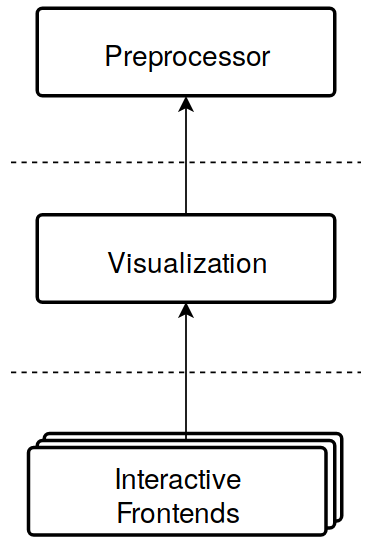
\includegraphics[width=0.5\textwidth]{img/module_design.png}
%         \caption{Submodules}
%         \label{fig:submodules}

%     \end{subfigure}% %this '%' is needed for side-by-side figure!
%     \begin{subfigure}{.7\textwidth}
%         \centering
%         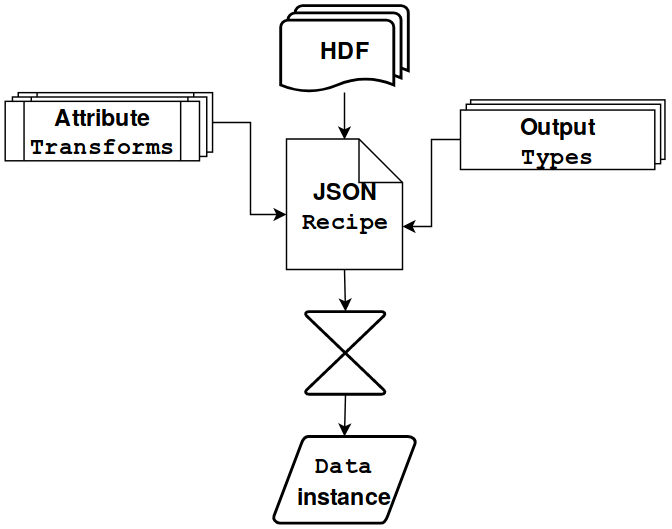
\includegraphics[width=0.7\textwidth]{img/reader_flowchart4.png}
%         \caption{Preprocessor}
%         \label{fig:preprocessor}
%     \end{subfigure}
%     \caption{Module Design.}
%     \label{fig:module-design}
% \end{figure}


\begin{figure}[htb!]
    % Fixed length
    \centering
    \subcaptionbox{Submodules\label{fig:submodules}}{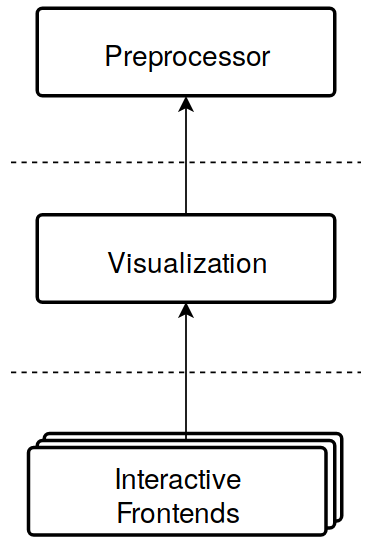
\includegraphics[width=1.6in]{img/module_design.png}}\hspace{5em}%
    \subcaptionbox{Preprocessor\label{fig:preprocessor}}{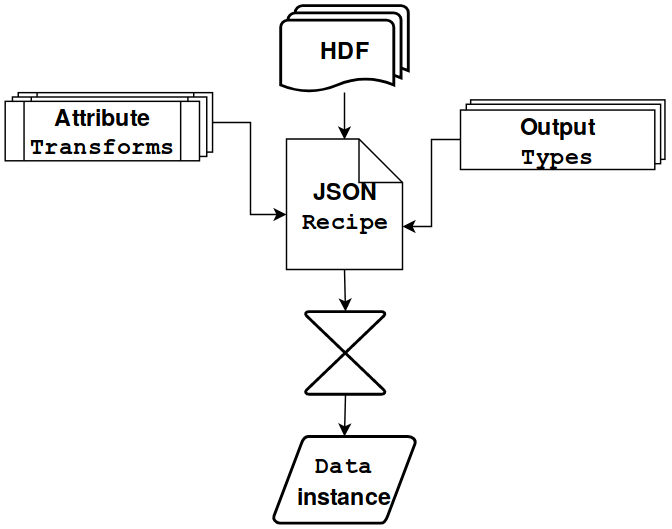
\includegraphics[width=0.5\textwidth]{img/reader_flowchart4.png}}
    \caption[Module Design.]{Module Design. The arrows indicate dependency in
      a), and dataflow in b).}
    \label{fig:module-design}
\end{figure}


\section{HDF Preprocessor Module}
\label{sec:preprocessor-module}

\subsection{Interface}
\label{sec:preprocessor-interface}

This is the 'backend' of the tool. It is basically a file reader for the input
data, for example a Fleur simulation output. Supported formats are the
Hierarchical Data Format (HDF) \cite{hdf} for the band structure, and a simple
Fleur-specific comma-separated values (CSV) format for the density of states
(DOS).

The HDF format is a flexible binary container for all kinds of common binary and
text file formats. Each file which constitutes a \texttt{Dataset} inside the HDF
file. The format supports metadata annotation and high-throughput input/output
(I/O). As a consequence, it is considered by developers in some application
domains that rely on numerical simulation codes, to arguably be one possible
base for the establishment of common domain-specific rich data exchange
standards in order to increase code interoperability. These developers are in
the process of extending their codes' I/O capabilities towards that end.
However, HDF's flexibility comes at the price of a relatively complex
Application Programming Interface (API) as the keyhole for all operations.

The preprocessor module serves as a wrapper around that API by introducing the
concept of \texttt{Recipes}, see Figure \ref{fig:preprocessor}. A specific
application \texttt{Recipe} is a dictionary that aims to describe a complete
\href{https://en.wikipedia.org/wiki/Extract,_transform,_load}{Extract-Transform-Load}
(ETL) pipeline for one specific application of the original data. The `extract'
is the reading of a dataset from HDF, the `transform' a sequence of once-through
functions applied to the the dataset, and the `load' the aggregation of all
transformed datasets into one runtime object which has all the methods for
operations on the data that are going to be used later on in the intended
application.

The `transform' and `output' type methods are defined in hierarchical
\texttt{Transform} and \texttt{Output\_Type} classes. Multiple inheritance is
used to sort them from general to application-specific applicability. This
structure is built using Python's \texttt{AbstractBaseClass} (\texttt{ABC}). The
advantages of the `recipes approach' are:
\begin{itemize}
\item All ETL processes for one application are collected in one simple list
    (the recipe), not locked in different code locations with conflicting
    contexts. In this list, entries can be sorted in any manner, e.g.
    alphabetical for perusal. Thus a recipe also serves as a concise
    documentation of how an application-domain HDF format should be handled.
\item Recipes are de/serializable (can be read from and saved to disk) and thus be
    machine-created and manipulated, for instance in a workflow pipeline.
\item The ETL processes, when declared in this interface, can be easily reused
    across applications. A recipe can combine different output types into a new
    type.
\end{itemize}

The feature that enables this flexibility is \textbf{type introspection}: the
preprocessor processes the datasets listed in the recipe in the order of their
mutual dependencies as found in the introspected listed transform and output
methods. When all transformed datasets have been added to the object, all
specified output types are searched and all their methods and attributes added.
Thus the output object's type is defined at runtime, when the preprocessing is
finished.

% \begin{figure}[htb!]
%     \centering
%     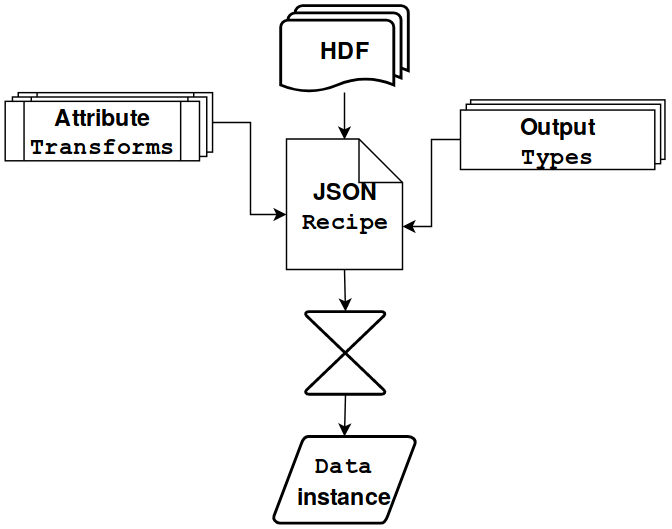
\includegraphics[width=0.6\textwidth]{img/reader_flowchart4.png}
%     \caption{The preprocessor module.}
%     \label{fig:preprocessor}
% \end{figure}

% \lstinputlisting[
% language=python,
% style=code,
% linerange=101-106
% captionpos=t,
% caption={Recipe \texttt{FleurBands} excerpt: dataset \texttt{BravaisMatrix}},
% label=recipe
% ]{listings/recipes.py}


\subsection{Implementation for Band Structure Visualization}
\label{sec:preprocessor-implementation}

The frontend has to draw three kinds of plots: a 3D atom plot of the unit cell
or supercell, and a combined band structure and DOS plot sharing the same
vertical energy axis. If no DOS data is present, the DOS part of the plot shall
be omitted. All three plots are controlled by one set of graphical frontend
control elements (widgets) for varying the parameters. In the current
implementation, the data for the first two plots come from a HDF file, while the
data for the DOS plot come from CSV files.

The band structure plot is a scatter plot. It plots discrete \(E(\mathbf{k})\)
data from the simulation. Firstly, the plotter needs the \(k\)-path (where
\(|\mathbf{k}|=k\)) for the horizontal axis. The preprocessor, having received
the recipe \texttt{FleurBands}, computes it from the \(k\)-points in the HDF in
a transform. Secondly, the plotter needs the eigenergies for every point on the
\(k\)-path, labeled by the band index \(\nu\), and its associated \(l\)-like
charge \(n_{s,k,\nu,g,l}\). This dataset is five-dimensional, and represents the
contribution of spin \(s\), \(k\)-point, band index \(\nu\),
atom group \(g\), and character or orbital \(l\) (here: only s,p,d,f) to the
specific eigenergy. So plotting must involve a dimension reduction. The
preprocessor resolves the processed data into the like-named output type
\texttt{FleurBands}. This type has a data selection method. The respective
\texttt{BandPlot} type calls this selector with a user selection of subsets of
all \((s,k,\nu,g,l)\). The method then computes the according \textbf{effective
  weight} shown in Equation \ref{eq:effective-weight}. The plotter uses that for
the dot size of each \(E(k)\) in the plot. Before rendering, the plotter
normalizes the energies to the Fermi Level.

\begin{align}
  W^{\text{eff}}_{s,k,\nu} = \left( \frac{\sum\limits_{\substack{g \in \text{groups} \\ l \in \text{characters}}} n_{s,k,\nu,g,l}\, N_g}{\sum\limits_{\substack{g \in \text{all groups} \\ l \in \text{all characters}}} n_{s,k,\nu,g,l}\, N_g} \right) \left(W_{s,k,\nu}^{\text{unf}}\right)^\alpha
\label{eq:effective-weight}
\end{align}

\(N_g\) denotes the number of atoms in a group. \(W_{s,k,\nu}^{\text{unf}}\) is
the unfolding weight, if the simulation was done with a supercell, and
\(\alpha\) its exponent. In the frontends, the latter is also a user control.
The effect of unfolding is illustrated in Figure \ref{fig:unfolding} for a toy
example of a monatomic chain, with a two-atom supercell of size \(a'\)
representing \(\alpha=0\) and a one-atom unit cell of size \(a\) representing
\(\alpha=1\). A use-case is discussed in the Application Chapter
\ref{chap:applications}.

\begin{figure}[htb!]
    \centering
    
\includegraphics[width=0.6\linewidth]{fig/unfolding.png}
    \caption[Band Unfolding]{Band unfolding: example for a simple monatomic
      chain. Adapted from \cite{hoffmann1987chemistry}.}
    \label{fig:unfolding}
\end{figure}

Even for small band structures, the selector has to access on the order \(10^7\)
individual data points for every selection change. Optimizations were introduced
which included:
\begin{itemize}
\item a cutoff filter that skips effective weights too small to show up on the
    plot,
\item use of optimized Numpy functions like \texttt{np.tensor} for the
    effective weight summation,
\item buffering of unchanged data between two selections,
\item array reshaping.
\end{itemize}

Together, these tweaks achieve a speedup of approximately \(10^2\) in plotting
speed. Thanks to that, the tool remains usable even when the input HDF is in the
\(10^2\) MB range.

\section{Visualization Module \& Interactive Graphical Frontends}
\label{sec:visualization-module}

\subsection{Visualization Module}
\label{sec:visualization-interface}

The Python visualization landscape abounds with a rapidly evolving plethora of
plotting libraries for different application contexts and technology stacks
\cite{python-viz-landscape}. Thus the project's visualization module's first
design objective was to account for that fact by decoupling it from any specific library
use, and modularizing it for intended applications. This structure again is built using Python's
\texttt{AbstractBaseClass} (\texttt{ABC}) interface and multiple inheritance.
Each application is represented by an abstract base class that contains the
common plotting method signatures. Likewise, each plotting library is represented by an
abstract base class that contains library-specifics. An \emph{implementation} inherits
both from one library base class and one or more application base classes. See
Fig. \ref{fig:visualization-module} for an impression. Thus switching the
library in a use context should require minimal adjustment, and a new
application (base class) can be be built from existing ones.

The second design objective was for the plotting methods to hide all
interactions with the actual plotting library used under the hood. The
application's base class' method arguments should only be tied to the data, not
the plotting library. Thus different frontend implementations need no or minimal
individual setup beforey they can call the same method for one specific plot
and receive the identical visualization with identical interactive behavior.

\begin{figure}[htb!]
    \centering
    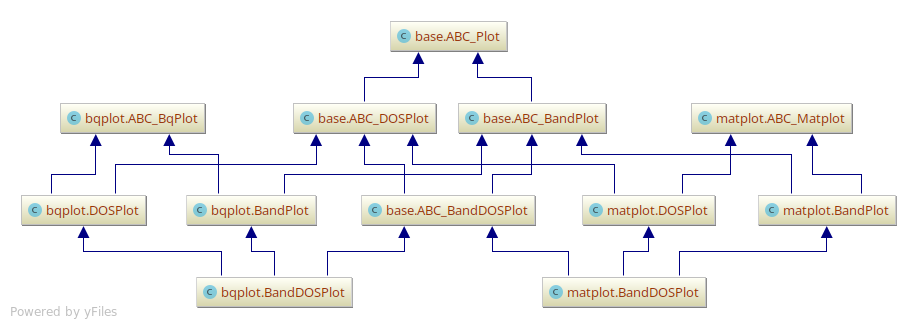
\includegraphics[width=1.0\linewidth]{img/pycharm_uml/matplot.png}
    \caption[Visualization Module Design]{Visualization Module Design: Example
      inheritance for two applications \texttt{BandPlot} and \texttt{DOSPlot}, and
      two plotting libraries \texttt{matplotlib} and \texttt{bqplot}.}
    \label{fig:visualization-module}
\end{figure}

\subsection{Desktop Frontend}
\label{sec:desktop-frontend}

A desktop frontend is always a helping hand for the physicists to just execute
it on the computer when one wants to go through the plots of the raw data that
is already in the computer.

Since the reading of HDF files and preprocessing of the data is done using
Python, it is decided that it would be best to also use Python for frontend
development. Considering various packages for frontend in python such as PyQt,
Tkinter and other libraries available for desktop GUIs, Tkinter is selected, as
it is bundled with Python and thus meets the requirement of easy maintainability
best. It is a package where every button can be designed and can be assigned to
a function. GUI types like \texttt{Label}, \texttt{Button},
\texttt{CheckButton}, \texttt{ListBox}, \texttt{Canvas} for plots, \texttt{Tab}
for viewing each plot in different tab have been used to make a simple desktop
frontend. It is simple to use with limited options for what the end-user, the
solid-state physicist, needs. It is also easy to convert the desktop frontend
code into a executable software and run in any system without any installation.

\subsection{Web Frontend}
\label{sec:web-frontend}

As web frontends continue to replace traditional desktop frontends in many
application domains \cite{web-vs-desktop}, so Python-based frontends and
visualizations are increasingly moving towards the browser, too. There, GUIs
with interactive visualizations are often called \textbf{Dashboards}. For this
project, a survey was undertaken to find the most suitable technology stack for
a web frontend. The full survey is documented in \cite{jw-notes}. The
requirements for the solution, on top of those stated in the introduction, were
defined as follows: The solution...

\begin{enumerate}
\item \textbf{openness}: relies solely on Open-Source-Software (OSS) with
    licensing suitable for academic use, has a stable release cycle, developer
    base and documentation,
\item \textbf{dashboarding}: features graphical control elements (widgets) that
    interact with InfoVis\footnote{InfoVis libraries: visualizations of
      information in arbitrary spaces, not necessarily the three-dimensional
      physical world. Example: matplotlib. SciVis libraries: visualizing
      physically situated data. Example: VTK \cite{python-viz-2018}.} plotting
    libraries,
\item \textbf{deployment}: ideally works like any web service, i.e. only a
    modern web browser is required to use it,
\item \textbf{maintenance}: requires only Python and no Web Development
    knowledge like e.g. Javascript, with respect to the product stakeholders.
\end{enumerate}

The last point implies a client-server model where the dashboard app is hosted
on a remote machine. This model requires a communication framework and protocol
between the Python interpreter running on the server and the JavaScript
interpreter running in the client browser. As per requirement no. 4, unlike a
generic Python web framework like e.g. \href{http://flask.pocoo.org/}{Flask},
the framework should take care of that communication by itself. Four major
frameworks were identified which fulfill the first three requirements:
\href{https://jupyter.org/}{Project Jupyter}, \href{http://pyviz.org/}{PyViz},
\href{https://bokeh.pydata.org/en/latest/}{Bokeh}, and
\href{https://plot.ly/products/dash/}{Dash by Plotly}. The last two only
partially fulfilled the requirement no. 4, so they were discarded. PyViz is the
newest contender among these four. Its expressed goal is to untangle the Python
visualization jungle by providing one high-level API that ties together all
major Python InfoVis libraries and data formats, including support for
dashboarding. This ambitious goal comes at the price of sacrificing support for
3D plotting \cite{pyviz-faq}, which was needed in this project for the atoms
plot. So PyViz had to be discarded.

This left Project Jupyter. By now, a wide variety of popular plotting libraries
have made their tools capable of working with Jupyter's widget library
\texttt{ipywidgets}. However, Jupyter only partially fulfills requirement no. 3
-- a Jupyter notebook (app) cannot, by itself, be published (deployed) as a
stand-alone website outside a live Jupyter environment \cite{python-viz-2018}:

\begin{quote}
    [...] ``However, despite their web-based interactivity, the ipywidgets-based
    libraries (ipyleaflet, pythreejs, ipyvolume, bqplot) are difficult to deploy
    as public-facing apps because the Jupyter protocol allows arbitrary code
    execution'' [...].
\end{quote}

To avoid requiring users to setup a working Jupyter environment on their
machine, the go-to solution for this problem is to setup a
\href{https://jupyter.org/hub}{JupyterHub} multi-user server. This still
requires users to register an account there, so it's not completely open.
Fortunately though, the intended users are contributors to the AiiDA project,
and so should have access to the JupyterHub-based \href{
  https://aiidalab.materialscloud.org/}{AiiDA Lab} service where the app can be
registered. Details on this procedure and alternative hosting solutions can be
found in the developer section of the manual \vref{for-developers}.


%%% Local Variables:
%%% mode: latex
%%% TeX-master: "../report"
%%% End:

%  LocalWords:  subpackages submodule frontend frontends backend
